\documentclass[12pt,a4paper]{article}

\usepackage[T1]{fontenc}
\usepackage{amsmath, amssymb, amsfonts}
\usepackage[magyar]{babel}
\usepackage[utf8]{inputenc}
\usepackage{graphicx}
\usepackage{graphics}
\usepackage{mathtools}
\usepackage{epsfig}
\usepackage{epstopdf}
\usepackage{cite}
\usepackage{caption}
\usepackage{hyperref}
\usepackage[bottom=4cm]{geometry}
%\geometry{a4paper, portrait, margin=1in}

\title{\huge{Korszerű vizsgálati módszerek labor jegyzőkönyv}\\ \vspace{20pt}
\textbf{Meissner-effektus mérése}}

\author{\Large{\textsc{Csörnyei Géza}} \vspace{10pt}\\
	\textrm{Eötvös Loránd Tudományegyetem}\\
	\textrm{Fizika BSc III. évfolyam}
	}
\date{}
%\lhead{}
\begin{document}
\addtolength{\voffset}{-1.0cm}
\addtolength{\textheight}{1.0cm}
\begin{titlepage}
\maketitle

\begin{figure}[!htb]
\centering

\includegraphics[scale=0.6]{eltecimer.jpg}
\end{figure}

\hfil \Large{'C' mérőcsoport}\hfil  \\
\vspace*{2pt}
\hfil \Large{\emph{Mérés dátuma:} 2018.04.26.}\hfil \\
\vspace*{2pt}
\hfil \hspace*{45pt} \Large{\emph{Mérés vezetője:} Dankházi Zoltán}\hfil
\thispagestyle{empty}
\end{titlepage}

\section{Bevezetés}
\hspace*{10pt} Mérésünk során megvizsgáltuk a szupravezető anyag esetében fellépő Meissner-effektust, majd meghatároztuk az anyag szuszceptibilitását. A laborgyakorlat során megismerkedtünk a lock-in műszer működésével és használatával, melyre a mérés érzékenységének növeléséhez és a zaj hatásának csökkentésére, vagyis a zaj által fedett jelek megjelenítéséhez volt szükség.

\section{Méréshez használt eszközök}
\hspace*{10pt} A mérésünkhöz használt eszközök közül a legfontosabb a lock-in berendezés volt, melynek lényege, hogy nagyon szűk sávszélességű tartományt mérve csökkenti a zajt, valamint növeli az érzékenységet. Ezt olyan módon éri el, hogy csak egy a rá adott referenciajel frekvenciáján érkező bemeneti jelek maradnak meg a hosszú időre vett átlagban, a többi jel eltűnik. A műszer elméletének ismertetése megtalálható [1]-ben. A műszer kapcsolási rajza a \ref{fig:1}. ábrán látható.\\
\begin{figure}[!h]
\centering
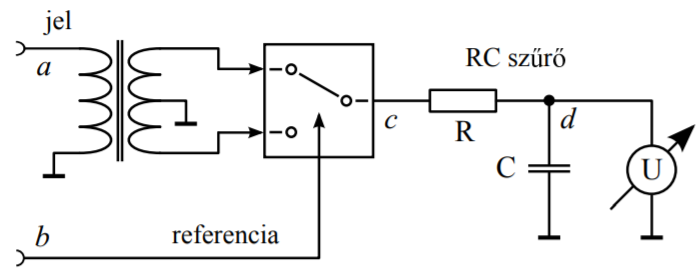
\includegraphics[scale=0.55]{lockin}
\caption{A lock-in műszer kapcsolási rajza}
\label{fig:1}
\end{figure}
\newline
\hspace*{10pt}A lock-in műszerre a referenciajelet egy frekvenciagenerátor segítségével adtuk. Ezen frekvenciagenerátor segítségével adtunk feszültséget a mérőfejre is, melynek mintát tartalmazó részét egy folyékony nitrogén által hűtött tartályba helyeztünk. A feszültséget DVM-el mértük, az adatok kimentését pedig számítógéppel végeztük. A mérési összeállítás megtalálható [1]-ben.

\section{Elméleti összefoglaló}
\hspace*{10pt} Szupravezetőnek nevezzük azon anyagokat, melyeket egy rájuk jellemző, kritikus hőmérséklet alá hűtve azok ellenállás gyakorlatilag nulla lesz. A Meissner-effektus lényege, hogy a kritikus hőmérséklet alá történő hűtés esetén a szupravezető anyagban eredetileg mérhető mágneses tér kiszorul belőle, vagyis az anyagban a mágneses indukció nulla lesz. Ekkor az anyag tökéletes diamágnes lesz, vagyis szuszceptibilitása $\chi=-1$ lesz. Ez azonban csak ideális esetben történik így, mivel az anyagnak csak egy része válik ténylegesen szupravezetővé. A minta szuszceptibilitását az összeállításban látható tekercseken mérhető feszültség minta jelenléte miatti megváltozásából lehet számolni az alábbi képlet segítségével:
$$\frac{\Delta U}{U_0}=-\chi \frac{V_m}{V},$$
ahol $U_0$ a minta nélküli esetben mérhető feszültség, $V_m$ a szupravezetővé váló minta térfogata, $V$ pedig a minta teljes térfogata. Esetünkben utóbbi két adat értékét [2]-ből olvastuk ki: $V_m=(22 \pm 0.22)$ mm$^{3}$ és $V=(300 \pm 3)$ mm$^3$.\\
\hspace*{10pt} A mérés megkezdése előtt először össze kellett illesztenünk a mért és a referencia jel fázisát, hogy a legerősebb jelet kaphassuk. Az beállítás után mérhető feszültségekre még rátevődött a műszer által adott offset jel, amely az előbbi beállítás során hasznos volt, ezen értéktől azonban számításainkhoz először meg kellett szabadulni. Ennek elérése érdekében megmértük a feszültséget 0$^{\circ}$ és 180$^{\circ}$-os fázistolás esetén, ekkor a kapott feszültségértékek egyikéből levonódott az offset feszültség, míg a másikhoz hozzáadódott (mivel az offset mindig egy irányba tolja a jelet, viszont a fázistolás előjelváltást eredményezett a bemeneti jelen, a differenciál erősítő miatt), így a két jel abszolútértékének  összegeként megkaphatjuk a valódi bemeneti feszültségértéket. A két mért érték -6.095 mV és 5.418 mV volt, így az átlaguk, ezáltal a keresett feszültségérték
$$U_0=-5.757 \pm 0.005 \textrm{ mV},$$
ahol a feszültségmérés hibájára a leolvasást és a beállítás bizonytalanságát figyelembe véve 0.1$\%$-os hibát becsültem.

\section{Kiértékelés}
\hspace*{10pt} A kalibrálás elvégzése után behelyeztük a mintát a nitrogénnel megtöltött tartályba, majd elindítottuk a mérés. Két mérést végeztünk, az első során a minta kritikus hőmérséklet alá történő hűlésének folyamatát, a másodikban, miután feljebb emeltük a mintatartót a tartályban, a visszamelegedés folyamatát vettük fel. A mérés során a minta hőmérsékletét egy a mintatartóban levő platina hőmérővel mértük. A kapott adatfájl tartalmazta az eltelt időt, a hőmérsékletet (mely nem pontosan a minta hőmérséklete volt, lévén egy hőmérő saját hőmérsékletét méri, és a hőmérő nem pontosan a minta mellett volt), valamint a lock-in feszültséget. A hűlés és a melegedés során felvett feszültségértékeket a hőmérséklet függvényében a \ref{fig:2}. ábrán ábrázoltam.
\newpage
\begin{figure}[!h]
\centering
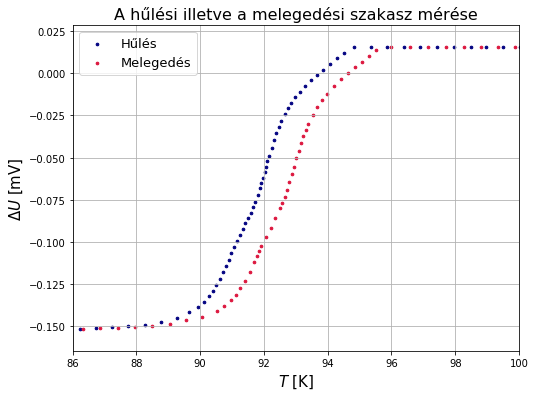
\includegraphics[scale=0.65]{hul_mel}
\caption{A mérés során kapott görbék}
\label{fig:2}
\end{figure}
A kapott ábrákon jól látszik, hogy a görbéknek hiszterézise van, mely [1] alapján a mintatartó véges hővezetéséből származik. Ezen hiszterézis kikompenzálható az [1]-ben leírtak alapján, ha a két görbe hőmérséklet szerinti átlagát vesszük. Az átlagolással kapott görbe a \ref{fig:3}. ábrán látható.
\begin{figure}[!h]
\centering
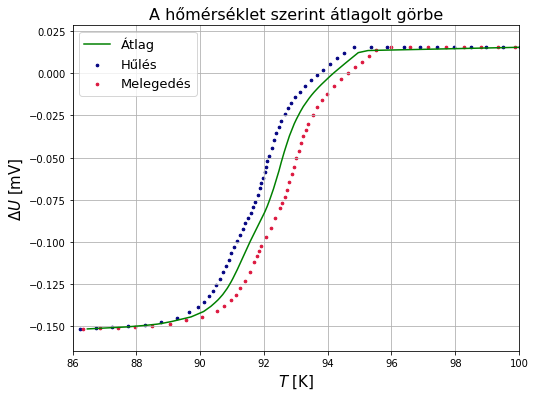
\includegraphics[scale=0.65]{atlag}
\caption{Az átlagolt görbe helyzete}
\label{fig:3}
\end{figure}
\newpage
Az így kapott görbe pontosságát az átalakulási sebességek figyelembevételével vizsgálhatjuk meg, mégpedig úgy, hogy az időadatok segítségével képezzük a melegedési illetve hűlési sebességeket és megnézzük, hogy a fenti eltolásokból származó hiba milyen arányban áll a mérés hibájával. A hőmérséklet és a hőmérsékletváltozás időfüggését a \ref{fig:4}. ábrán ábrázoltam.\\
\begin{figure}[!h]
\centering
\hspace*{-1cm}
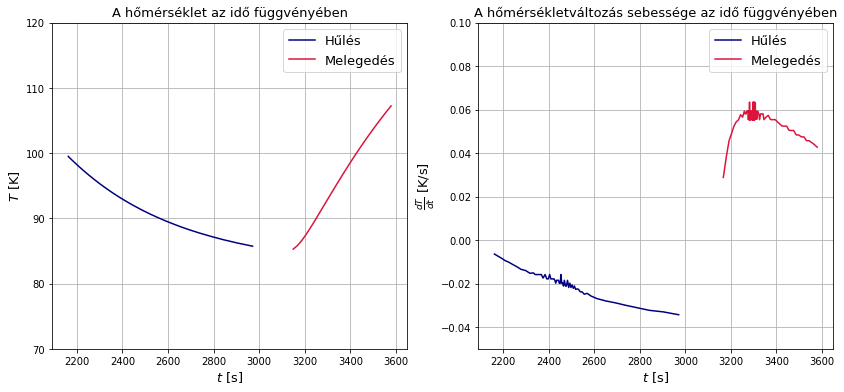
\includegraphics[scale=0.55]{hom_valt}
\caption{A hőmérséklet és annak változási sebességének időfüggése a hűlés és melegedés esetére}
\label{fig:4}
\end{figure}
\newline
Ezt követően a hőmérsékletváltozás sebességének (annak abszolút értékének) megfelelő súlyokkal átlagoltam össze a hűlési és melegedési görbéket, a kapott görbe a \ref{fig:5}. ábrán látható.
\newpage
\begin{figure}[!h]
\centering
\hspace*{-1cm}
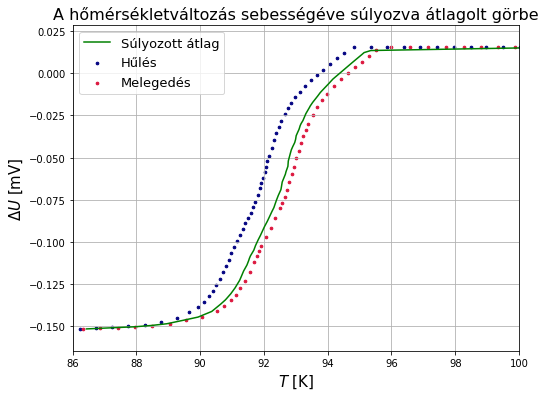
\includegraphics[scale=0.65]{sulyozott}
\caption{A hőmérsékletváltozás sebességére súlyozott átlaggörbe}
\label{fig:5}
\end{figure}
Ha összevetjük ezen görbét a korábban, tisztán az átlagolással kapott görbével, akkor látható, hogy elég nagy az eltérés. A továbbiakban ezen görbével fogunk dolgozni, ezt használjuk fel a szuszceptibilitás meghatározására.
\begin{figure}[!h]
\centering
\hspace*{-1cm}
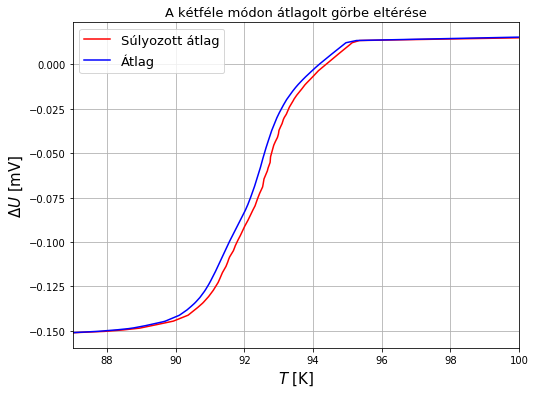
\includegraphics[scale=0.65]{elteres}
\caption{A két átlaggörbe eltérése}
\label{fig:6}
\end{figure}
\newpage
A fenti görbe segítségével ki tudjuk számolni a szuszceptibilitás hőmérsékletfüggését is. Ehhez a fenti képletet használtam, melybe behelyettesítettem az ismert, illetve számolt értékeket, így lényegében csak a lock-in feszültségeket kellett egy számolt konstanssal szoroznom, hogy megkapjam a szuszceptibilitás értékeket. Az így kapott hőmérséklet-szuszceptibilitás görbe a \ref{fig:7}. ábrán látható.\\
\begin{figure}[!h]
\centering
\hspace*{-1cm}
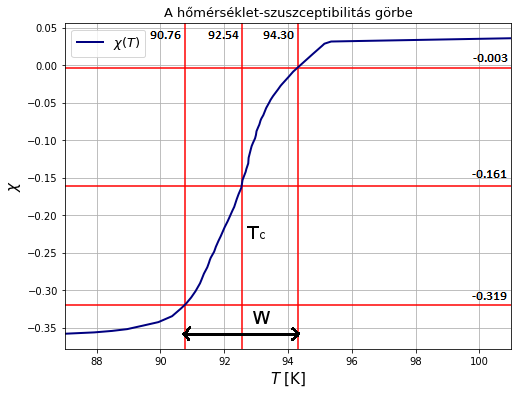
\includegraphics[scale=1.15]{szusz}
\caption{A szuszceptibilitás hőmérsékletfüggése. Az ábrán bejelöltem a fázisátalakulás hőmérsékletét ($T_c$), az $50\%$-os szuszceptibilitásérték megkeresésével, valamint az átalakulás szélességét, a $10\%$-os, illetve a $90\%$-os szuszceptibilitásérték megkeresésével.}
\label{fig:7}
\end{figure}
\newline
Az ábráról is leolvasható, hogy a minta szuszceptibiliása a fázisátalakulás után
$$\chi = -0.358 \pm 0.013 $$
lesz, ahol a hibát mind a hőmérsékletmérés becsült hibája ($\approx 0.5$ K), mind a mérési statisztikus hiba (0.001 mV, melyet a fázisátalakulás utáni $\Delta U$ értékek szórásából állapítottam meg) figyelembevételével adtam meg. A kapott érték értelemszerűen nagyobb mint -1, ugyanis nem a teljes minta, csupán annak egy része vált szupravezetővé. A minta kritikus hőmérséklete az ábráról leolvashatóan 
$$T_c=92.54 \pm 0.5 \textrm{ K},$$
az átalakulás szélessége pedig
$$W=3.54 \pm 0.01 \textrm{ K} .$$

\newpage
\section{Diszkusszió}
\hspace*{10pt} Mérésünk során megismerkedtünk a Meissner-effektus méréséhez szükséges berendezésekkel, megfigyeltünk egy anyag szupravezetővé történő alakulásának folyamatát, és meghatároztuk a szupravezető szuszceptibilitását, valamint kritikus hőmérsékletét.

\section*{Hivatkozások}
\hspace*{14pt} [1] : \emph{Kiadott jegyzet}:\\
\hspace*{34pt} \texttt{http://atomfizika.elte.hu/kvml/docs/korszeruosszefuzott.pdf}\\
\hspace*{14pt} [2] : \emph{Mérési információk}:\\
\hspace*{34pt} \texttt{http://austen.elte.hu/adatok/MEISNER/info.txt}

\section*{Mérési jegyzetre vonatkozó megjegyzések}
\hspace*{10pt} A mérési leírással kapcsolatosan egy megjegyzéssel szeretnék élni: a hőmérséklet változás sebességégével való súlyozás szükségességét, illetve a hibaszámítás mibenlétét nem világította meg számomra kellőképpen a jegyzet, nem értettem milyen hibaszámítási eljárás kellett volna ahhoz, hogy bebizonyosodjék, hogy a szimpla átlaggörbe nem a legjobb leírása a fázisátalakulásnak. Hasznosnak érezném ezen részhez a kívánt hibaszámítás részletezését, illetve azt, hogy milyen határ elérése esetén szükséges a sebességekkel történő súlyozás.

\end{document}